\section{Analogue Input}

In this section you will learn how to read in analogue input.
The numbers aren't true analogue, just 1024 possible values.
Here you will be reading off a voltage compared to 5V.


\setlength{\tabcolsep}{0pt}
\begin{center}
\begin{tabular}{|c| c |}
\hline
    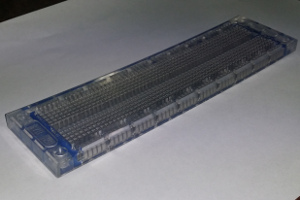
\includegraphics[align=c,width=0.2\textwidth]{./Graphics/breadboard}
    & 
    \begin{minipage}[t]{0.2\textwidth}
        \centering
        1 $\times$ Bread Board 
    \end{minipage}\\ \hline
    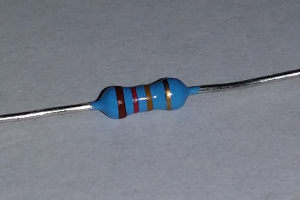
\includegraphics[align=c,width=0.2\textwidth]{./Graphics/12k_resistor} 
    & 1 $\times$ 12K$\Omega$ Resistor \\ \hline
    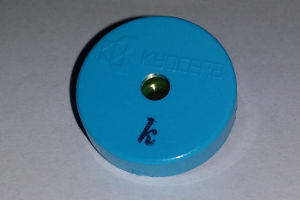
\includegraphics[align=c,width=0.2\textwidth]{./Graphics/piezo}
    & 1 $\times$ Piezo\\ \hline
    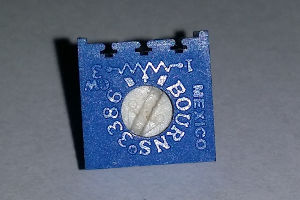
\includegraphics[align=c,width=0.2\textwidth]{./Graphics/pot}
    & 1 $\times$ Potentiometer\\ \hline
    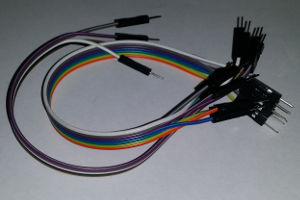
\includegraphics[align=c,width=0.2\textwidth]{./Graphics/jumper_cables}
    & 2 $\times$ Jumper Cables \\ \hline
  \end{tabular}
\end{center}

\begin{center}
    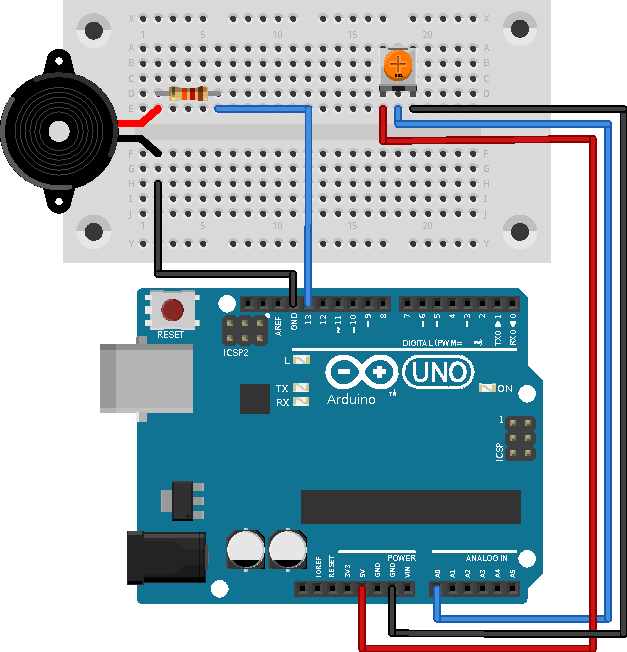
\includegraphics[width=0.4\textwidth]{./Graphics/piezo_circuit}
\end{center}

The important circuit here is the one with the pot.
The other one with the piezo is just there to give you feedback
on the value that's being read.

\begin{center}
    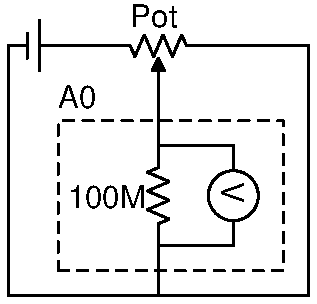
\includegraphics[width=0.2\textwidth]{./Graphics/PotCircuit.pdf}
    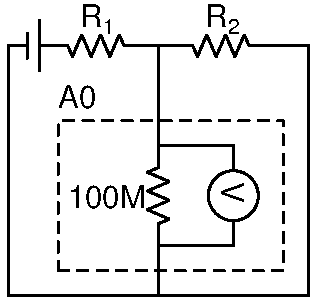
\includegraphics[width=0.2\textwidth]{./Graphics/PotEquivCircuit.pdf}
\end{center}

The equivalent circuit from which you will read off the voltage.
Explain more of the physics.

\subsection{Hardware}
\subsubsection{Potentiometer}
\begin{center}
    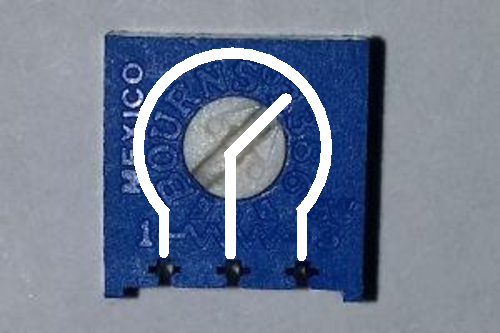
\includegraphics[width=0.2\textwidth]{./Graphics/pot_internal}
\end{center}

The potentiometer, 
pot for short,
is a variable resistor.
By connecting the thing you already ground it
so you can't get tristate logic,
if you just connect live and input you will only get noise even when its off.

You control it by turning the knob in the middle.

\subsubsection{Piezo}

This is an element that shrinks and expends when a voltage is applied.
This produces noise.

\subsection{Software}

\lstinputlisting[style=Arduino]{./Src/piezo.src}
Tone is half duty cycle unsigned unsigned int,
can overflow.


